% dvisvgm --pdf name
% latexmk -C
\documentclass[preview]{standalone}
\usepackage{tikz}
\usepackage{amsmath}
\usetikzlibrary{shapes.geometric, arrows}
\tikzstyle{block} = [rectangle, rounded corners,
minimum width=3cm,
minimum height=1cm,
text centered, 
draw=gray]

\tikzstyle{io} = [trapezium, 
trapezium stretches=true,
trapezium left angle=70, 
trapezium right angle=110, 
minimum width=3cm, 
minimum height=1cm, text centered, 
draw=gray]

\tikzstyle{process} = [rectangle, 
minimum width=3cm,
minimum height=1cm,
text centered, 
text width=3cm, 
draw=gray]

\tikzstyle{decision} = [diamond, 
minimum width=3cm, 
minimum height=1cm, 
text centered, 
draw=gray]
\tikzstyle{arrow} = [thick,->,>=stealth]

\tikzstyle{circle} = [circle, 
minimum size=1cm, 
text centered, 
draw=gray]

\begin{document}
    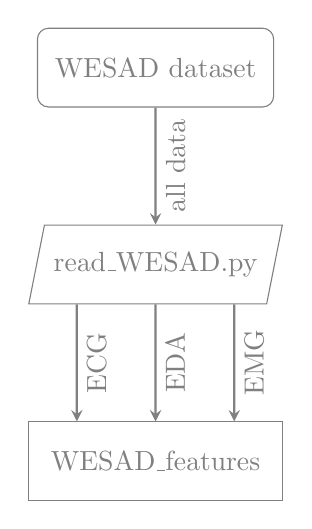
\begin{tikzpicture}[transform shape, every node/.append style={}, color=gray, node distance = 2.5cm]
        \node (WESAD) [block] {WESAD dataset};
        \node (read_WESAD) [io, below of=WESAD] {read\_WESAD.py};
        \node (wesad_features) [process, below of = read_WESAD] {WESAD\_features};

        \draw [arrow] (WESAD) -- node[midway, rotate=90, below] {all data} (read_WESAD);
        \draw [arrow] ([xshift=-1cm]read_WESAD.south) -- node[midway, rotate=90, below] {ECG} ([xshift=-1cm]wesad_features.north);
        \draw [arrow] (read_WESAD) -- node[midway, rotate=90, below] {EDA} (wesad_features);
        \draw [arrow] ([xshift=1cm]read_WESAD.south) -- node[midway, rotate=90, below] {EMG} ([xshift=1cm]wesad_features.north);
    \end{tikzpicture}
\end{document}